\documentclass[11pt,notes]{beamer}
\usetheme{Boadilla}

%\usepackage{pgfpages}
\usepackage[utf8]{inputenc}
\usepackage[T1]{fontenc}
\usepackage{graphicx}
\usepackage{bbding}
\usepackage{ textcomp }
\usepackage{color}
\usepackage{pgf}
\usepackage{tikz}
\usetikzlibrary{arrows,automata,positioning}

\setbeamertemplate{caption}[]

\newcommand*\tick{\item[\Checkmark]}
\newcommand*\fail{\item[\XSolidBrush]}
\newcommand*\prog{\item[\textgreater]}
\newcommand*\fstar{\item[\FiveStar]}

\author{Simon Schlepphorst, Federico Diaz Capriles}
\title{Ising Model}
\subtitle{A Statistical System at Finite Temperature}

\logo{\includegraphics[height=1.5cm]{Images/logo}\vspace{220pt}}

\institute{Uni Bonn}

\date{16 March 2017}

\setbeamercovered{transparent}

\setbeamertemplate{navigation symbols}{}









\begin{document}
	

\begin{frame}
	\titlepage
\end{frame}

\begin{frame}
	\tableofcontents
\end{frame}

\section{Introduction}
\subsection{Theory}
\begin{frame}
	\frametitle{Introduction}
	\framesubtitle{Theory}
	\begin{minipage}{.6\textwidth}
			\begin{center}
			
\begin{tikzpicture}
				\draw[step=.5cm,gray,very thin] (0.1,0.1) grid (2.9,2.9);
				\fill[black] (0.1,0.1) rectangle (.5,1.5);
				\fill[black] (0.1,1.5) rectangle (2,2);
				\fill[black] (2,0.1) rectangle (2.5,0.5);
				\fill[black] (1.5,0.5) rectangle (2,1);
				\fill[black] (0.5,1) rectangle (1,1.5);
				\fill[black] (2,2) rectangle (2.9,2.9);
			\end{tikzpicture}
		\end{center}
	\end{minipage}%
	\begin{minipage}[]{.4\textwidth}
		$ \square $ Spin up \\ 
		$ \blacksquare $ Spin down 
	\end{minipage}
	\vspace{-.05cm}
	\begin{equation}
		 \mathcal{H}(\textbf{s}) = -J \sum_{\langle i, j \rangle} s_{i} s_{j}
	\end{equation}
	{\scriptsize \begin{equation*}
		 s_{n} \in \{-1,+1\}
	\end{equation*}}\vspace{-.5cm}
	\begin{equation}
		\textbf{s} = (s_{1}, s_{2}, \dots, s_{N})
	\end{equation}
	\begin{equation}
		\mathcal{Z} = \sum_{\textbf{s}} exp(-\frac{1}{k_{B} T}\mathcal{H}(s))
	\end{equation}
	
\note{
1. Describe graphic\\
2. Hamiltonian of the system. This is the $\mathcal{H}$ with no external field.\\
\ \ \ J in this case denotes which type of interaction we have in our lattice:\\
\ \ \ J > 0 $ \rightarrow $ Ferromagnetic $ \rightarrow $ Spins want to be alligned\\
\ \ \ J < 0 $ \rightarrow $ Antiferromagnetic $ \rightarrow $ Spins want opposite of neighbors\\
\ \ \ J = 0 $ \rightarrow $ Noninteracting\\
3. Canonical Partition function. It would take a lot of time to go into detail on the Partition function (PF); but in a nutshell, it describes the statistical properties of the system and it represents a particular statistical ensemble. \\
}
\end{frame}

\subsection{Monte Carlo Motivation}
\begin{frame}
\frametitle{Introduction}
\framesubtitle{Monte Carlo Motivation}
Ising model can be difficult to evaluate numerically if there are many states for the system. For example, let:\\
\begin{description}
	\item[L:] Total number of sites in the lattice (length $\times$ width)
	\item[$s_{j}$:] Spin state of the j-th point ($s_{n} \in \{-1,+1\}$)
\end{description}
With 2 states per spin, we have a total of $2^{L}$ possible configurations.\\
$\hookrightarrow$ Want to use Monte Carlo Methods
\begin{description}
	\item[What can we find with MC?] Estimates on the properties of the lattice
	\item[What does MC do?] Use random number generation and accept reject\\ \ \ \ \ \ \ \ \ \ methods to simulate lattice interaction
\end{description}
\note{
Some properties that can be estimated are: Specific heat or magnetization (at a given temperature)
}
\end{frame}
\subsection{Markov Chains}
\begin{frame}
\frametitle{Introduction}
\framesubtitle{Markov Chains}\vspace{-.5cm}
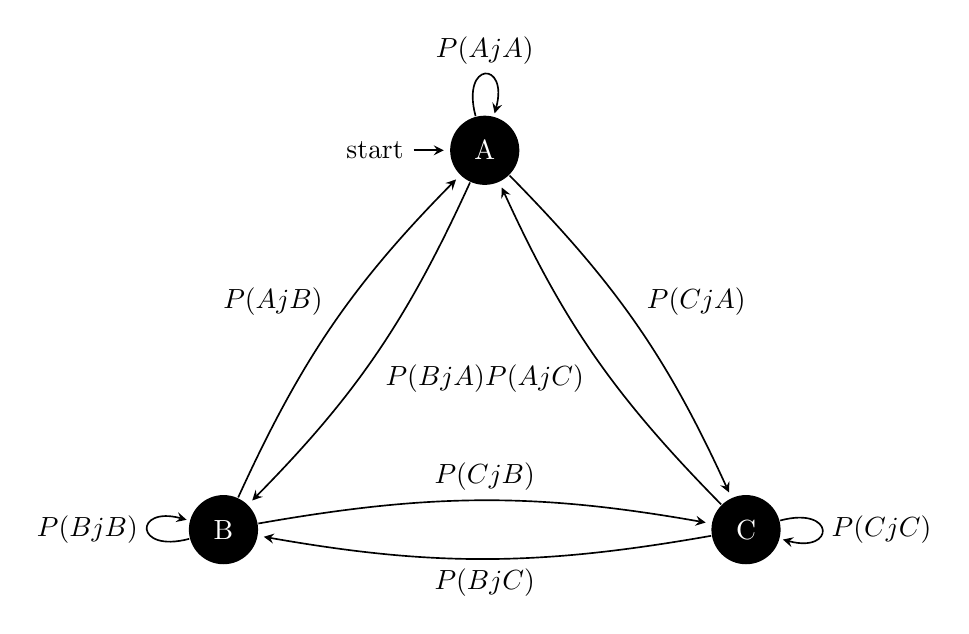
\begin{tikzpicture}[->,>=stealth,shorten >=2pt,auto,node distance=5cm,
semithick]

\tikzstyle{every state}=[fill=black,draw=none,text=white]

\node[initial, state]         (A)                    {A};
\node[state]                  (B) [below left=4.5cm and 3cm]  {B};
\node[state]                  (C) [below right=4.5cm and 3cm] {C};

\path (A) edge [loop above] node {${P(A\textbar A)}$} (A)
          edge [bend left=10] node {${P(B\textbar A)}$} (B)                    
          edge [bend left=10] node {${P(C\textbar A)}$} (C)
      (B) edge [loop left]  node {${P(B\textbar B)}$} (B)
          edge [bend left=10] node {${P(C\textbar B)}$} (C)
          edge [bend left=10] node {${P(A\textbar B)}$} (A)
      (C) edge [loop right] node {${P(C\textbar C)}$} (C)
          edge [bend left=10] node {${P(A\textbar C)}$} (A)
          edge [bend left=10] node {${P(B\textbar C)}$} (B);
\end{tikzpicture}
\note{
Markov Chains are mathematical systems that hop from one "state" (a situation or set of values) to another. That is to say, Markov chains tell you the probability to transition between states in a system. \\
So what takes us from state A to (lets say) state C is a series of jumps relying on probability. \\
}
\end{frame}
\begin{frame}
We can build a matrix P which will be a stochastic matrix which will then be used to describe the probability for any initial state, $\mu$, to go to a final state, $\nu$. 

\[\begin{bmatrix}
	P_{11} & P_{12} & P_{13} &    \dots    & P_{1m} \\
	P_{21} & P_{22} & P_{23} &    \dots    & P_{2m} \\
	\vdots & \vdots & \vdots & P_{\mu \nu} & \vdots \\
	P_{n1} & P_{n2} & P_{n3} &    \dots    & P_{nm}
\end{bmatrix}\vspace{.5cm}\]
In the figure you can see a simple Markov Chain of 3 states. Furthermore, it is worth noting that $\sum_{s'} P(s'\textbar s) = 1$\\ 
We have a probability $ P(y\textbar x) \equiv P(x\rightarrow y) $

\note{
We have prob for state x to go to y 
}
\end{frame}
\subsection{Metropolis Algorithm}
\begin{frame}
\frametitle{Introduction}
\framesubtitle{Metropolis Algorithm}
\begin{itemize}
	\item 
\end{itemize}


\note{

}
\end{frame}






\end{document}